\documentclass[letterpaper]{article}
%\documentclass[a5paper]{article}

%% Language and font encodings
\usepackage[english]{babel}
\usepackage[utf8x]{inputenc}
\usepackage[T1]{fontenc}

%% Sets page size and margins
\usepackage[letterpaper,top=.75in,bottom=1in,left=1in,right=1in,marginparwidth=1.75cm]{geometry}
%\usepackage[a5paper,top=1cm,bottom=1cm,left=1cm,right=1.5cm,marginparwidth=1.75cm]{geometry}

\usepackage{graphicx}
%\graphicspath{../images}	  %%where to look for images

%% Useful packages
\usepackage{amssymb, amsmath, amsthm} 
%\usepackage{graphicx}  %%this is currently enabled in the default document, so it is commented out here. 
\usepackage{calrsfs}
\usepackage{braket}
\usepackage{mathtools}
\usepackage{lipsum}
\usepackage{tikz}
\usetikzlibrary{cd}
\usepackage{verbatim}
%\usepackage{ntheorem}% for theorem-like environments
\usepackage{mdframed}%can make highlighted boxes of text
%Use case: https://tex.stackexchange.com/questions/46828/how-to-highlight-important-parts-with-a-gray-background
\usepackage{wrapfig}
\usepackage{centernot}
\usepackage{subcaption}%\begin{subfigure}{0.5\textwidth}
\usepackage{pgfplots}
\pgfplotsset{compat=1.13}
\usepackage[colorinlistoftodos]{todonotes}
\usepackage[colorlinks=true, allcolors=blue]{hyperref}
\usepackage{xfrac}					%to make slanted fractions \sfrac{numerator}{denominator}
\usepackage{enumitem}            
    %syntax: \begin{enumerate}[label=(\alph*)]
    %possible arguments: f \alph*, \Alph*, \arabic*, \roman* and \Roman*
\usetikzlibrary{arrows,shapes.geometric,fit}

\DeclareMathAlphabet{\pazocal}{OMS}{zplm}{m}{n}
%% Use \pazocal{letter} to typeset a letter in the other kind 
%%  of math calligraphic font. 

%% This puts the QED block at the end of each proof, the way I like it. 
\renewenvironment{proof}{{\bfseries Proof}}{\qed}
\makeatletter
\renewenvironment{proof}[1][\bfseries \proofname]{\par
  \pushQED{\qed}%
  \normalfont \topsep6\p@\@plus6\p@\relax
  \trivlist
  %\itemindent\normalparindent
  \item[\hskip\labelsep
        \scshape
    #1\@addpunct{}]\ignorespaces
}{%
  \popQED\endtrivlist\@endpefalse
}
\makeatother

%% This adds a \rewnewtheorem command, which enables me to override the settings for theorems contained in this document.
\makeatletter
\def\renewtheorem#1{%
  \expandafter\let\csname#1\endcsname\relax
  \expandafter\let\csname c@#1\endcsname\relax
  \gdef\renewtheorem@envname{#1}
  \renewtheorem@secpar
}
\def\renewtheorem@secpar{\@ifnextchar[{\renewtheorem@numberedlike}{\renewtheorem@nonumberedlike}}
\def\renewtheorem@numberedlike[#1]#2{\newtheorem{\renewtheorem@envname}[#1]{#2}}
\def\renewtheorem@nonumberedlike#1{  
\def\renewtheorem@caption{#1}
\edef\renewtheorem@nowithin{\noexpand\newtheorem{\renewtheorem@envname}{\renewtheorem@caption}}
\renewtheorem@thirdpar
}
\def\renewtheorem@thirdpar{\@ifnextchar[{\renewtheorem@within}{\renewtheorem@nowithin}}
\def\renewtheorem@within[#1]{\renewtheorem@nowithin[#1]}
\makeatother

%% This makes theorems and definitions with names show up in bold, the way I like it. 
\makeatletter
\def\th@plain{%
  \thm@notefont{}% same as heading font
  \itshape % body font
}
\def\th@definition{%
  \thm@notefont{}% same as heading font
  \normalfont % body font
}
\makeatother

%===============================================
%==============Shortcut Commands================
%===============================================
\newcommand{\ds}{\displaystyle}
\newcommand{\B}{\mathcal{B}}
\newcommand{\C}{\mathbb{C}}
\newcommand{\F}{\mathbb{F}}
\newcommand{\N}{\mathbb{N}}
\newcommand{\R}{\mathbb{R}}
\newcommand{\Q}{\mathbb{Q}}
\newcommand{\T}{\mathcal{T}}
\newcommand{\Z}{\mathbb{Z}}
\renewcommand\qedsymbol{$\blacksquare$}
\newcommand{\qedwhite}{\hfill\ensuremath{\square}}
\newcommand*\conj[1]{\overline{#1}}
\newcommand*\closure[1]{\overline{#1}}
\newcommand*\mean[1]{\overline{#1}}
%\newcommand{\inner}[1]{\left< #1 \right>}
\newcommand{\inner}[2]{\left< #1, #2 \right>}
\newcommand{\powerset}[1]{\pazocal{P}(#1)}
%% Use \pazocal{letter} to typeset a letter in the other kind 
%%  of math calligraphic font. 
\newcommand{\cardinality}[1]{\left| #1 \right|}
\newcommand{\domain}[1]{\mathcal{D}(#1)}
\newcommand{\image}{\text{Im}}
\newcommand{\inv}[1]{#1^{-1}}
\newcommand{\preimage}[2]{#1^{-1}\left(#2\right)}
\newcommand{\script}[1]{\mathcal{#1}}


\newenvironment{highlight}{\begin{mdframed}[backgroundcolor=gray!20]}{\end{mdframed}}

\DeclarePairedDelimiter\ceil{\lceil}{\rceil}
\DeclarePairedDelimiter\floor{\lfloor}{\rfloor}

%===============================================
%===============My Tikz Commands================
%===============================================
\newcommand{\drawsquiggle}[1]{\draw[shift={(#1,0)}] (.005,.05) -- (-.005,.02) -- (.005,-.02) -- (-.005,-.05);}
\newcommand{\drawpoint}[2]{\draw[*-*] (#1,0.01) node[below, shift={(0,-.2)}] {#2};}
\newcommand{\drawopoint}[2]{\draw[o-o] (#1,0.01) node[below, shift={(0,-.2)}] {#2};}
\newcommand{\drawlpoint}[2]{\draw (#1,0.02) -- (#1,-0.02) node[below] {#2};}
\newcommand{\drawlbrack}[2]{\draw (#1+.01,0.02) --(#1,0.02) -- (#1,-0.02) -- (#1+.01,-0.02) node[below, shift={(-.01,0)}] {#2};}
\newcommand{\drawrbrack}[2]{\draw (#1-.01,0.02) --(#1,0.02) -- (#1,-0.02) -- (#1-.01,-0.02) node[below, shift={(+.01,0)}] {#2};}

%***********************************************
%**************Start of Document****************
%***********************************************

%===============================================
%===============Theorem Styles==================
%===============================================

%================Default Style==================
\theoremstyle{plain}% is the default. it sets the text in italic and adds extra space above and below the \newtheorems listed below it in the input. it is recommended for theorems, corollaries, lemmas, propositions, conjectures, criteria, and (possibly; depends on the subject area) algorithms.
\newtheorem{theorem}{Theorem}
\numberwithin{theorem}{section} %This sets the numbering system for theorems to number them down to the {argument} level. I have it set to number down to the {section} level right now.
\newtheorem*{theorem*}{Theorem} %Theorem with no numbering
\newtheorem{corollary}[theorem]{Corollary}
\newtheorem*{corollary*}{Corollary}
\newtheorem{conjecture}[theorem]{Conjecture}
\newtheorem{lemma}[theorem]{Lemma}
\newtheorem*{lemma*}{Lemma}
\newtheorem{proposition}[theorem]{Proposition}
\newtheorem*{proposition*}{Proposition}
\newtheorem{problemstatement}[theorem]{Problem Statement}


%==============Definition Style=================
\theoremstyle{definition}% adds extra space above and below, but sets the text in roman. it is recommended for definitions, conditions, problems, and examples; i've alse seen it used for exercises.
\newtheorem{definition}[theorem]{Definition}
\newtheorem*{definition*}{Definition}
\newtheorem{condition}[theorem]{Condition}
\newtheorem{problem}[theorem]{Problem}
\newtheorem{example}[theorem]{Example}
\newtheorem*{example*}{Example}
\newtheorem*{counterexample*}{Counterexample}
\newtheorem*{romantheorem*}{Theorem} %Theorem with no numbering
\newtheorem{exercise}{Exercise}
\numberwithin{exercise}{section}
\newtheorem{algorithm}[theorem]{Algorithm}

%================Remark Style===================
\theoremstyle{remark}% is set in roman, with no additional space above or below. it is recommended for remarks, notes, notation, claims, summaries, acknowledgments, cases, and conclusions.
\newtheorem{remark}[theorem]{Remark}
\newtheorem*{remark*}{Remark}
\newtheorem{notation}[theorem]{Notation}
\newtheorem*{notation*}{Notation}
%\newtheorem{claim}[theorem]{Claim}  %%use this if you ever want claims to be numbered
\newtheorem*{claim}{Claim}



\pgfplotsset{compat=1.13}

%\newcommand{\T}{\mathcal{T}}
%\newcommand{\B}{\mathcal{B}}
\newcommand{\arbcup}[1]{\bigcup\limits_{\alpha\in\Gamma}#1_\alpha}
\newcommand{\arbcap}[1]{\bigcap\limits_{\alpha\in\Gamma}#1_\alpha}
\newcommand{\Rbad}{\R_\text{bad}}

\title{Math 501 \linebreak
Homework 9}
\author{Trevor Klar}

\begin{document}

\maketitle

\begin{enumerate}
\item A space $X$ is called \emph{functionally normal} if for all pairs of disjoint closed sets $A$ and $B$ in $X$, there is a continuous function $f:X\to [0,1]$ with $f(a)=0$ for all $a\in A$ and $f(b)=0$ for all $b\in B$. 

Prove that if $X$ is functionally normal, then $X$ is normal. 

\begin{proof}
Suppose $X$ is functionally normal, and let $A$ and $B$ be two disjoint closed sets in $X$. Consider $\preimage{f}{[0,\frac{1}{\pi})}$. Since $f$ is continuous and $[0,\frac{1}{\pi})$ is open in $[0,1]$, then $\preimage{f}{[0,\frac{1}{\pi})}$ is open in $X$. Since $f(a)=0$ for all $a\in A$, then $A\subset\preimage{f}{[0,\frac{1}{\pi})}$. Similarly, $B\subset \preimage{f}{(\frac{2}{\pi},1]}$. Since $f$ is continuous and $[0,\frac{1}{\pi})\cap (\frac{2}{\pi},1]=\emptyset$, then $\preimage{f}{[0,\frac{1}{\pi})}\cap \preimage{f}{(\frac{2}{\pi},1]}=\emptyset$. 

Thus, for all disjoint sets $A$ and $B$ in $X$, there exist disjoint open sets $\preimage{f}{[0,\frac{1}{\pi})}$ and $\preimage{f}{(\frac{2}{\pi},1]}$ such that $A \subset \preimage{f}{[0,\frac{1}{\pi})}$ and $B\subset \preimage{f}{(\frac{2}{\pi},1]}$. 
\end{proof}

\item Let $X$ be a space. Prove that $X$ is normal if and only if for any closed set $A$ and open set $U$ with $A \subset U$, there is an open set $V$ with $A \subset V \subset \closure{V} \subset U$.

\begin{center}
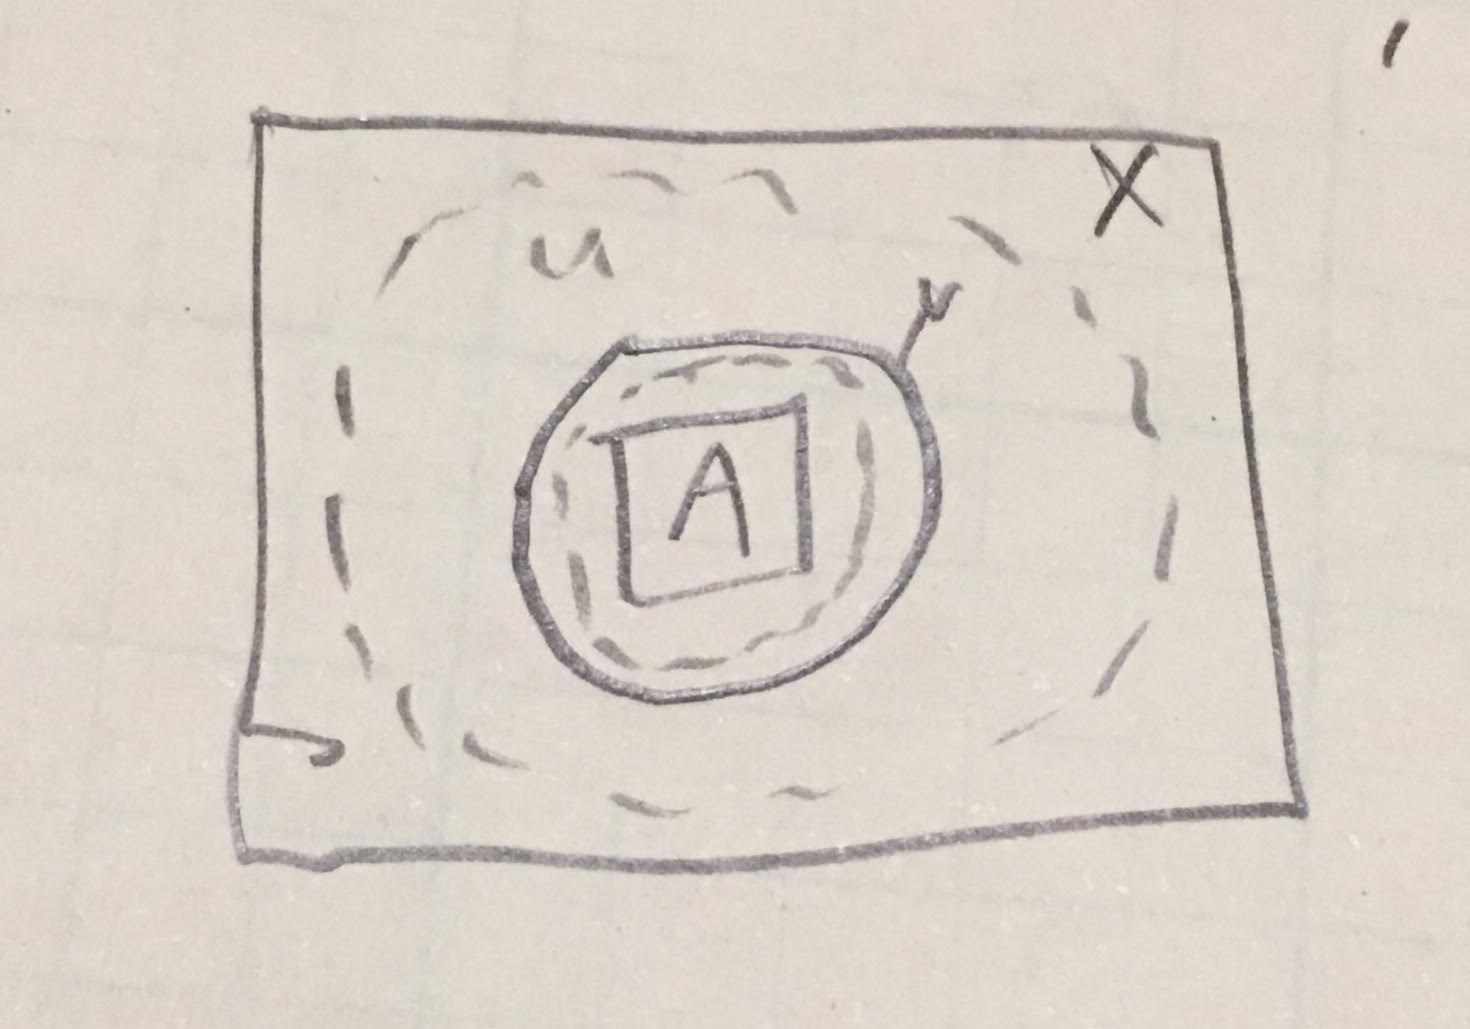
\includegraphics[scale=.1]{hw9_prob2_forward}
\end{center}

\begin{proof}($\implies$)
Let $X$ be normal, with $A$ closed and $U$ open such that $A\subset U$. Consider the closed set $U^\complement=X-U$. Since $A\subset U$, then $A\cap U^\complement = \emptyset$. Now since $X$ is normal, there exist open sets $V,V'$, with $A\subset V$, $U^\complement\subset V'$, and $V\cap V'=\emptyset$. Currently, we have shown that $A\subset V\subset U$. 

\textit{Claim:} $\closure{V}\cap V'=\emptyset$. \\
To see this, suppose for contradiction that $x\in\closure{V}\cap V'$. Now, $x\not\in V\cap V'$, because $V\cap V'=\emptyset$. So, $x\in V^\ell\cap V'$. Since $x$ is a limit point of $V$ and $V'$ is an open set containing $x$, then $V\cap(V'-\{x\})\neq\emptyset$, which is a contradiction. \qedwhite

Since $\closure{V}\cap V' = \emptyset$, then $\closure{V}\cap U^\complement = \emptyset$, so $\closure{V}\subset U$. Thus, 
$A\subset V\subset \closure{V}\subset U.$
\end{proof}
\pagebreak

\begin{center}
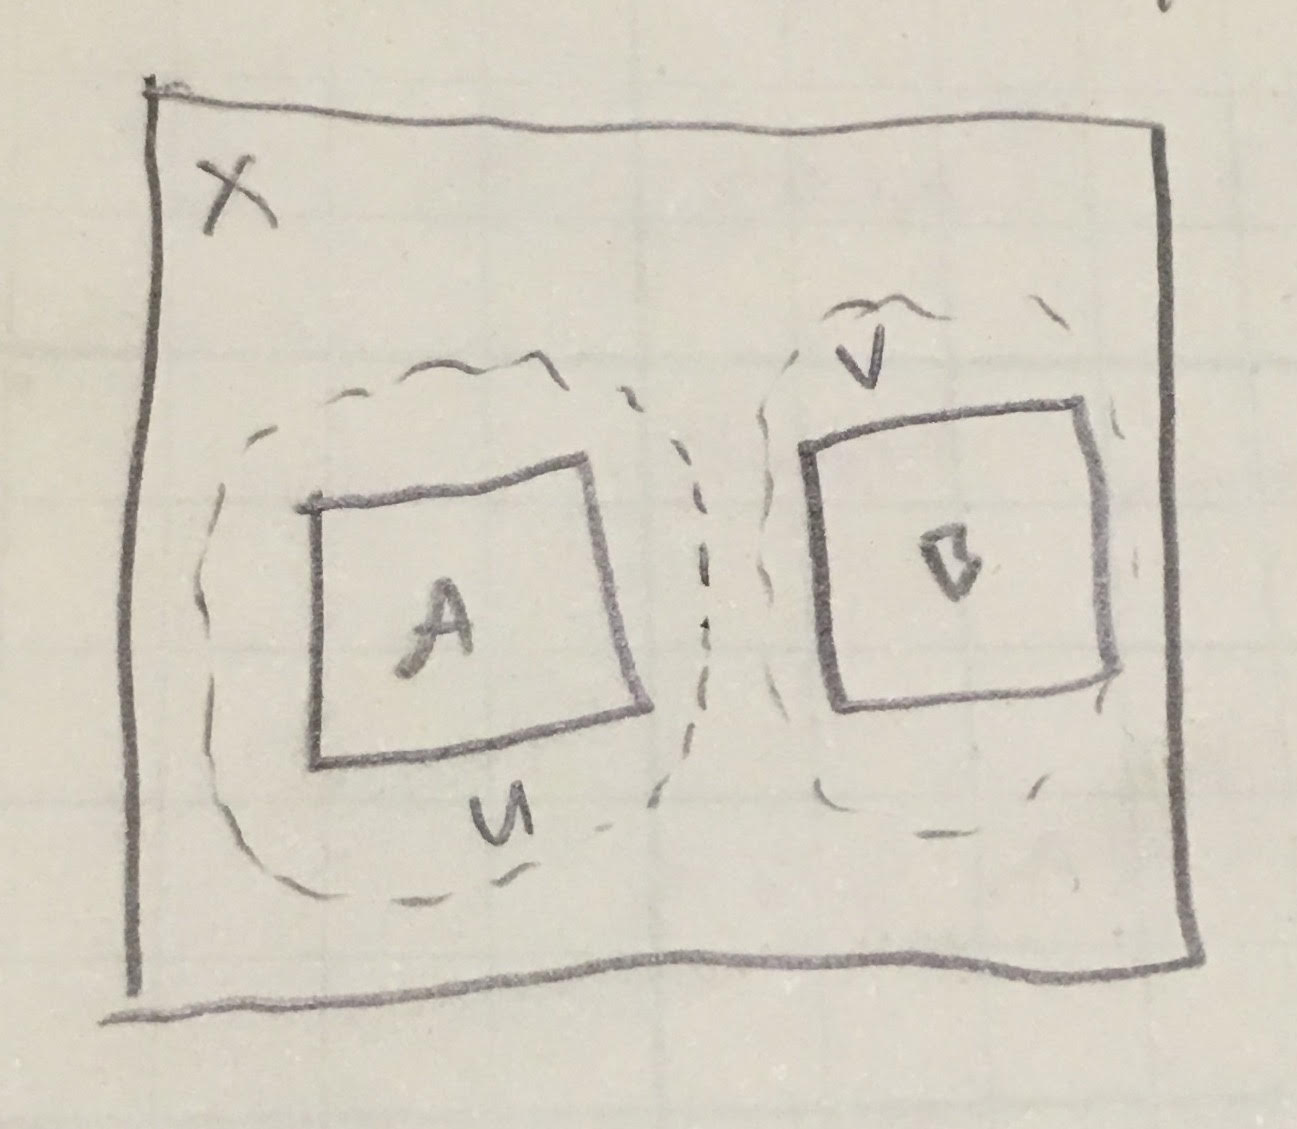
\includegraphics[scale=.1]{hw9_prob2_converse}
\end{center}

\begin{proof}($\impliedby$)
Suppose that for any closed set $A$ and open set $U$ with $A \subset U$, there is an open set $V$ with $A \subset V \subset \closure{V} \subset U$. Let $A$ and $B$ be closed sets in $X$ with $A\cap B=\emptyset$.

Since $A\subset B^\complement$, and $B^\complement$ is open, then there exists an open set $U$ with $A\subset U\subset \closure{U}\subset B^\complement$. Similarly, since $B\subset \closure{U}^\complement$, and $\closure{U}^\complement$ is open, then there exists an open set $V$ with $B\subset V \subset \closure{V}\subset \closure{U}^\complement$. Since $V\subset \closure{U}^\complement$, then $V\cap \closure{U}=\emptyset$, so $V\cap U=\emptyset$. 

Thus, $A\subset U$, $B\subset V$, and $U\cap V=\emptyset$. 
\end{proof}

\item Let $X$ be a normal space. Prove for each pair of disjoint closed sets $A$ and $B$, there are disjoint open sets $U$ and $V$ with $A \subset U$, $B \subset V$, and $\closure{U} \cap \closure{V} = \emptyset$.
\begin{proof}
Let $A$ and $B$ be closed sets in $X$ with $A\cap B=\emptyset$. By exercise (2)($\implies$), since $X$ is normal, it satisfies the hypotheses for (2)($\impliedby$). By (2)($\impliedby$), there exist open sets $U,V$ such that $A \subset U$, $B \subset V$, and $\closure{V} \subset \closure{U}^\complement$. Thus, $\closure{U} \cap \closure{V} = \emptyset$ and we are done. 
\end{proof}

\item Prove that the Tietze Extension Theorem implies Urysohn’s Lemma. (Remark: There exist proofs of the
Tietze Extension Theorem which do not rely on Urysohn’s Lemma. Thus the Tietze Extension Theorem
and Urysohn’s Lemma are equivalent.)

\begin{center}
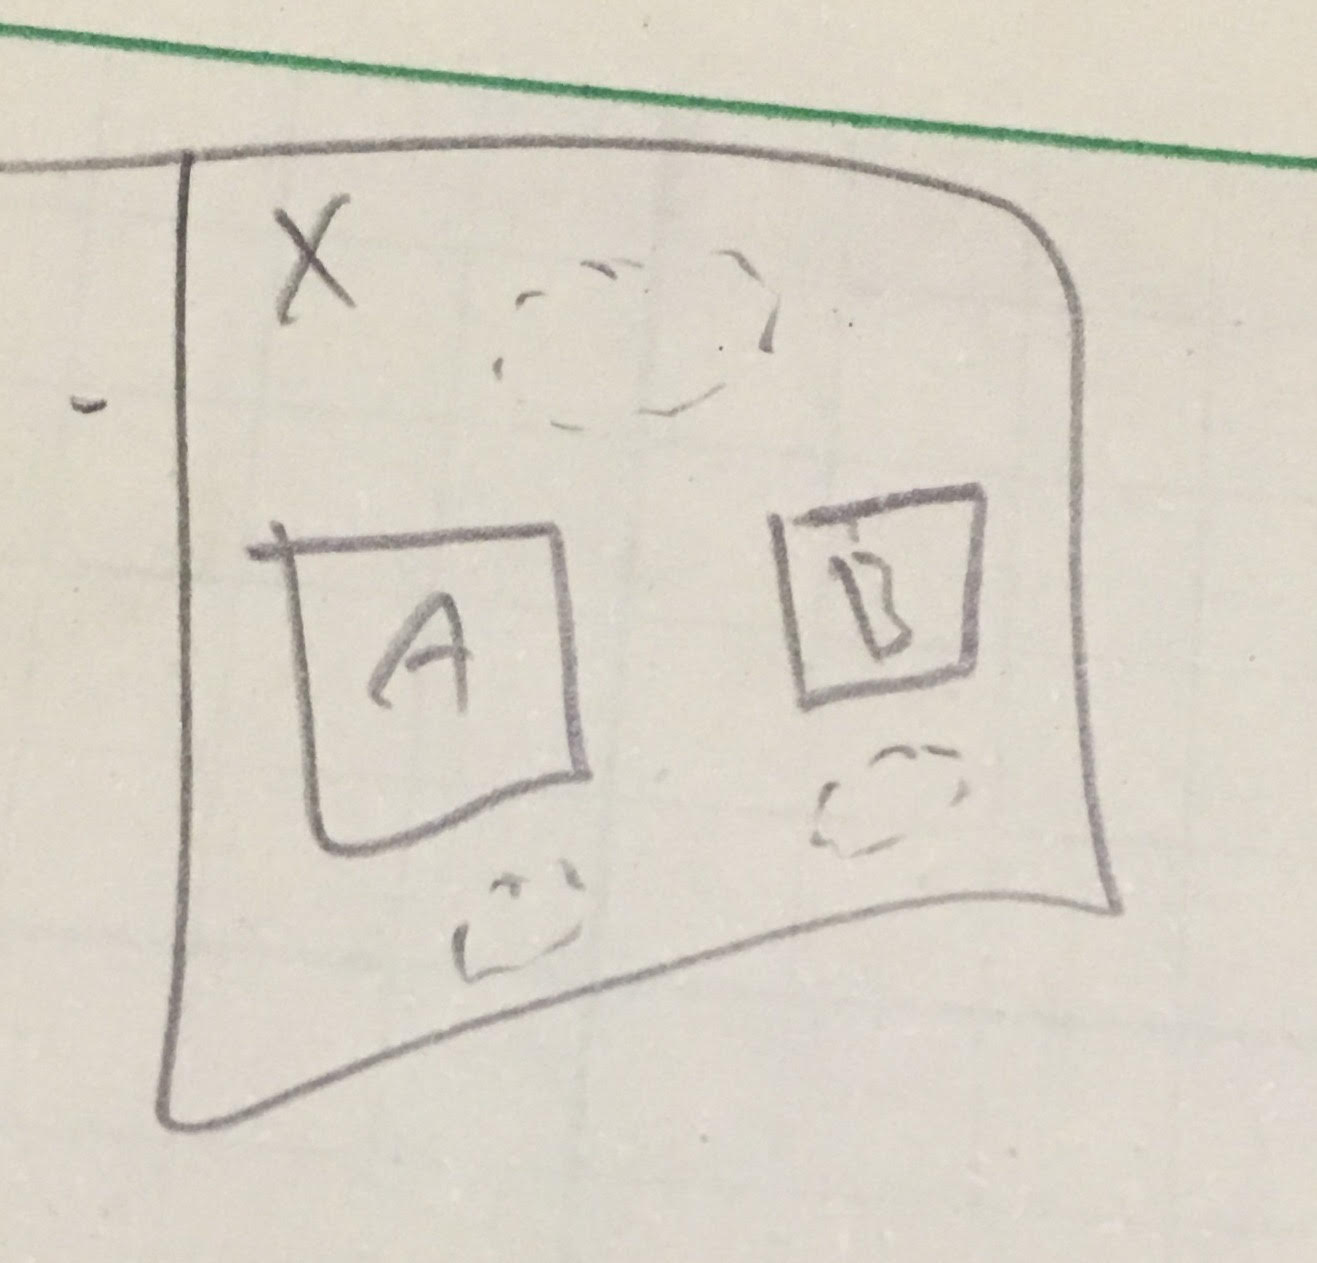
\includegraphics[scale=.07]{hw9_prob4}
\end{center}

\begin{proof}
Let $X$ be a normal space, with $A,B$ disjoint closed subsets of $X$. We will prove that there exists a continuous function $\varphi: X \to [0,1]$ such that $\varphi(a)=0$ for all $a \in A$, and $\varphi(b)=1$ for all $b \in B$.

Let $S = A \cup B$. Let $f:S\to \R$ be 
\[\begin{array}{rr}
f(a) = 0 & \forall a\in A\\
f(b) = 1 & \forall b\in B.\\
\end{array}\]
Now, $f|_A$, $f|_B$ are constant functions on compact domains, so they are continuous. Thus, by the Piecing Lemma, $f$ is continuous. Now, by Tietze's Extension Theorem, there exists a continuous function $F:X\to \R$ such that $f(x)=F(x)$ for all $x\in S$. 

Now, define $\varphi: X \to [0,1]$ by 
$$\varphi(x)=
\begin{cases}
0 & F(x)\leq 0\\
F(x) & F(x)\in[0,1]\\
1 & F(x)\geq 1\\
\end{cases}_.$$
Note that since $F$ is continuous, $\preimage{F}{(-\infty, 0]}$ and $\preimage{F}{[1,\infty)}$ are closed. So, since $\varphi$ is constant on the above closed sets, it is continuous on them, and it is equivalent to the continuous function $F$ on $[0,1]$. Thus, by the Piecing Lemma, $\varphi$ is continuous. Therefore, we have shown that there exists continuous $\varphi: X \to [0,1]$ such that $\varphi(a)=0$ for all $a \in A$, and $\varphi(b)=1$ for all $b \in B$.
\end{proof}

\item Let $X$ be a compact Hausdorff space, and let ${\{U_\alpha\}_{\alpha\in\Gamma}}$ be an open cover of X. Prove that there exists a finite subcover $U_{\alpha_1}, \ldots, U_{\alpha_n}$ of $X$ and a collection of functions $\varphi_{\alpha_1}, \ldots, \varphi_{\alpha_n}: X \to [0,1]$ such that

\begin{enumerate}[label=(\roman*)]
\item For each $i = 1,...,n$, there exists a compact set $K_{\alpha_i} \subset U_{\alpha_i}$ such that $\varphi	_{\alpha_i}(x)=0$ for $x \in X - K_{\alpha_i}$;
\item For each $x\in X, \sum\limits_{i=1}^n \varphi_{\alpha_i}(x) = 1$. 
\end{enumerate}
(Remark: The $\varphi_{\alpha_i}$ and $U_{\alpha_i}$ are called a \emph{partition of unity subordinate to the cover} $\{U_\alpha\}$. Hints: $X$ is normal. Use Urysohn’s Lemma to find functions $f_{\alpha_i}$ satisfying (i.). Let $\varphi_{\alpha_i} = \frac{f_{\alpha_i}}{\sum_j f_{\alpha_j}}$.)

\begin{center}
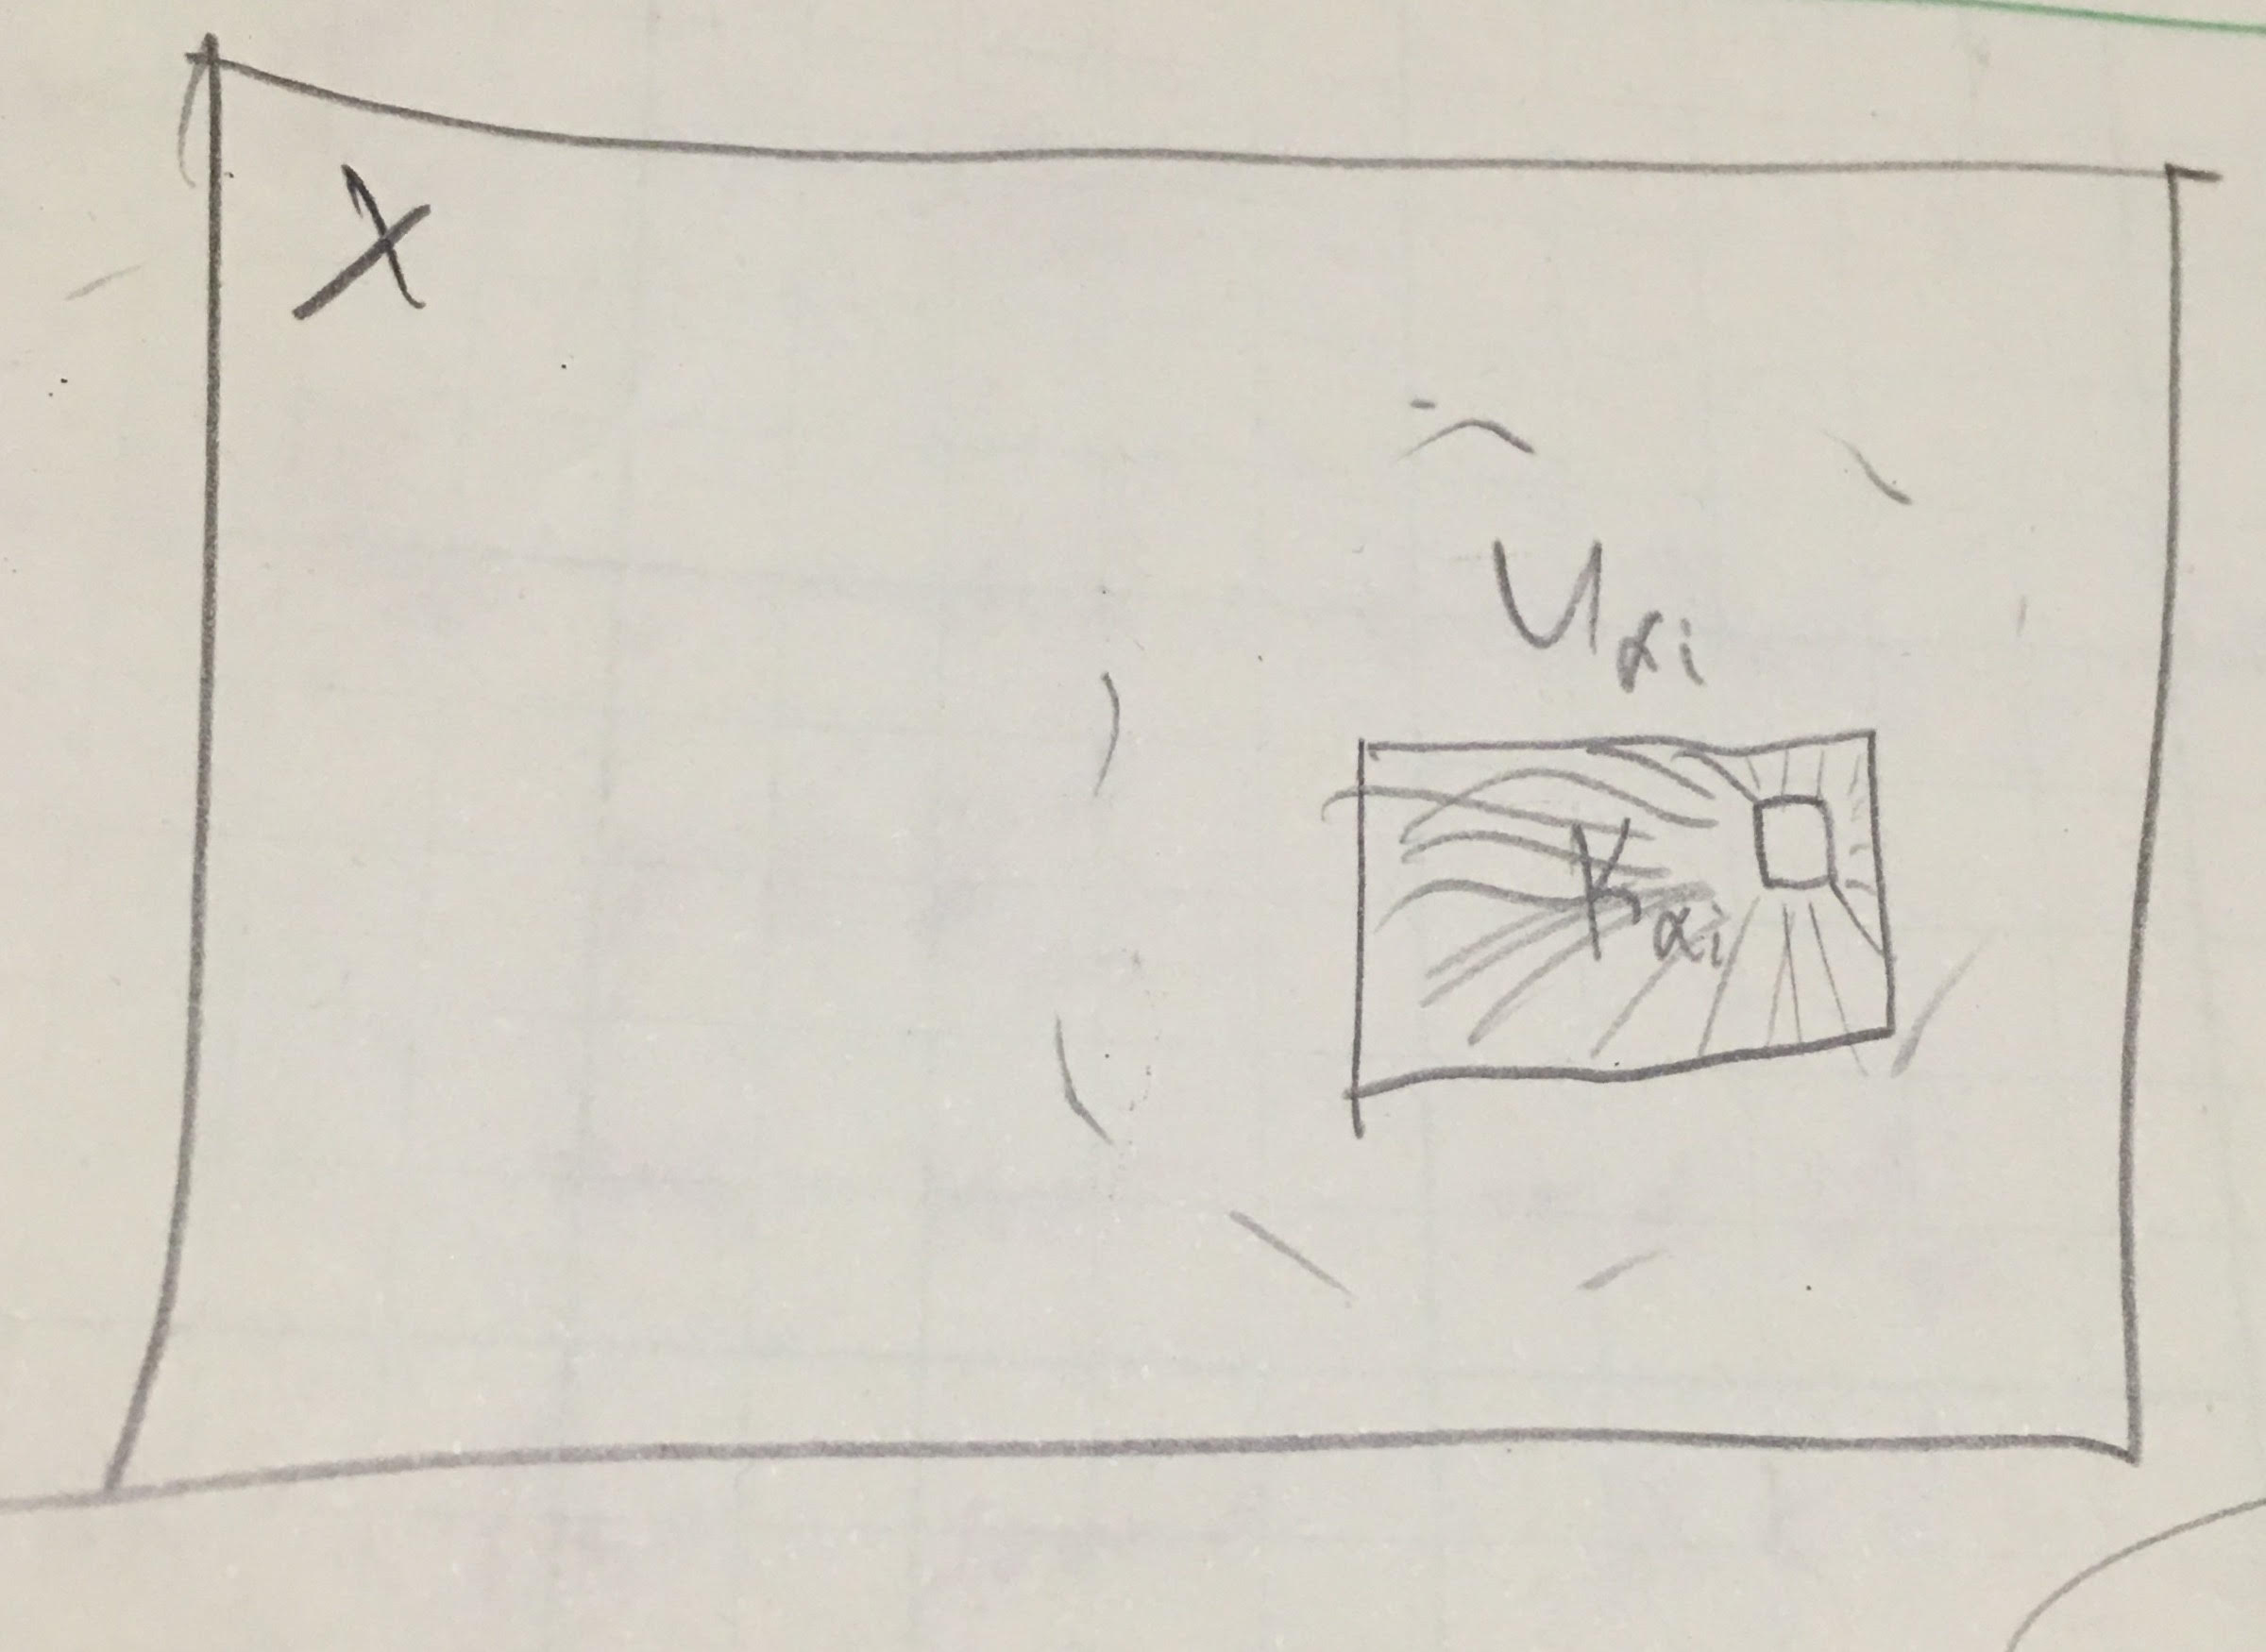
\includegraphics[scale=.07]{hw9_prob5}
\end{center}

\begin{proof} \textbf{of (i)}
Since $X$ is compact, then there exists a finite subcover $\{U_{\alpha_i}\}_{i=1}^n$. Let $\{K_{\alpha_i}\}_{i=1}^n$ be a collection of closed sets such that for each $i\in\{1, \ldots, n\}$, 
$$K_{\alpha_i} \subset U_{\alpha_i},$$
and $\{K\alpha_i\}_{i=1}^n$ covers $X$.
%\emph{Claim:} $K_{\alpha_i}$ is closed (and therefore compact), for every $i\in\{1, \ldots, n\}$. \\
%Choose some $j\in \{1, \ldots, n\}$. Let $x\in K_{\alpha_j}^\ell$, and suppose for contradiction that $x\not\in K_{\alpha_j}$. Then, $x\not\in U_{\alpha_j}$. Since $\{U_{\alpha_i}\}_{i=1}^n$ covers $X$, then $x\in U_{\alpha_k}$ for some $k\neq j$. Thus, $U_{\alpha_k}$ is an open set containing $x$ such that $U_{\alpha_k}-\{x\}\cap K_{\alpha_j} = \emptyset$, which contradicts the assumption that $x\in K_{\alpha_j}^\ell$. \qedwhite
Let $\{V_{\alpha_i}\}_{i=1}^n$ be closed sets with $V_{\alpha_i} \subset \text{int}(K_{\alpha_i}) \subset K_{\alpha_i}$ for each $i\in\{1, \ldots, n\}$ (We know that these closed sets exists because $X$ is Hausdorff, so even a singleton is closed).
%Let $K_{\alpha_i}=\closure{\widetilde{K}}_{\alpha_i}$ and let $\widetilde{K}^\complement_{\alpha_i} = X-\widetilde{K}_{\alpha_i}$, for simplicity.
Now, $X-\text{int}(K_{\alpha_i})$ and $V_{\alpha_i}$ are both closed and $X-\text{int}(K_{\alpha_i}) \cap V_{\alpha_i} = \emptyset$ for every $i\in\{1, \ldots, n\}$. This means that by Urysohn's Lemma, for each $i\in\{1, \ldots, n\}$, there exists a continuous function $f_{\alpha_i} :X\to\R$ such that
$$
f_{\alpha_i}(x)= 
\begin{cases}
0 \quad \quad \text{if} &x \in X-\text{int}(K_{\alpha_i})\\
>0 \quad \text{if} &x \in \text{int}(K_{\alpha_i})\\
1 \quad \quad \text{if} & x\in V_{\alpha_i}\\
\end{cases}
$$
Thus, we have (i), since $f_{\alpha_i}(x)=0$ for all $x\in X-\text{int}(K_{\alpha_i})$, and $(X-K_{\alpha_i})\subset (X-\text{int}(K_{\alpha_i}))$.
\end{proof}
\begin{proof} \textbf{of (ii)}
For each $i\in\{1, \ldots, n\}$, let $\varphi : X \to [0,1]$ be 
$$\varphi_{\alpha_i} = \frac{f_{\alpha_i}}{\sum_{j=1}^n f_{\alpha_j}}_\textbf{.}$$
\textit{Remark:} Since $\{K\alpha_j\}_{j=1}^n$ covers $X$, then for all $x\in X$, there exists some $k\in\{1, \ldots, n\}$ such that $x\in \text{int}(K\alpha_k)$. Thus, $\sum\limits_{j=1}^n f_{\alpha_j} \neq 0$, and so $\varphi_{\alpha_i}$ is defined everywhere.

Thus, $\{\varphi_{\alpha_i}\}_{i=1}^n$ satisfies (i) and (ii), since $f_{\alpha_i}(x)=0 \iff \varphi_{\alpha_i}(x)=0$, and 
$$\sum_{i=1}^n \varphi_{\alpha_i} = \sum_{i=1}^n \left( \frac{f_{\alpha_i}}{\sum_{j=1}^n f_{\alpha_j}} \right) = \frac{\sum_{i=1}^n f_{\alpha_i}}{\sum_{j=1}^n f_{\alpha_j}} \equiv 1.$$
\end{proof}
\end{enumerate}

\end{document}
